\documentclass[../piano_di_qualifica.tex]{subfiles}
\begin{document}
\subsection{Primo periodo (RR)}
\label{sub:periodo-RR}
\paragraph{Risultati test fase di analisi}
Qui di seguito verranno presentati i resoconti relativi ai test effettuati nella fase di analisi. \par

\begin{table}[!ht]
	\centering
	\begin{tabular}{|p{4cm}|p{4cm}|l|c|c|}
		\hline
		\rowcolor{lightgray}
		\textbf{Obiettivo}            			& \textbf{Metrica}              & \textbf{Risultato}                    & \textbf{Accettabile} & \textbf{Esito} \\
		\hline
		QPR01 Ritardo maturato        			& MPR02 Varianza pianificazione & 14 giorni                             & \(\leq 4\)           & Non Superato   \\
		QPR02 Budget parziale intaccato        	& MPR03 Varianza costi          & superiore al 5\%									& 0\%                  & Non Superato   \\
		QPR02.2 Budget finale intaccato        	& MPR03 Varianza costi          & Budget totale intatto					& 0\%                  & Superato       \\
		QPR05 Rispetto obiettivi      			& MPR07 Obiettivi soddisfatti   & 100\%                                 & 100\%                & Superato       \\
		QPR09 Rispetto delle norme   			& MPR08 Norme rispettate        & 100\%                                 & 100\%                & Superato       \\
		QPR12 Verifica documenti      			& MPR10 Frequenza controllo     & Ogni Milestone e modifica         	& Ogni Milestone       & Superato       \\
		OQP01 Leggibilità testo       			& MQP01 Indice di Gulpease      & 79,3                                  & \(\ge 60\)           & Superato       \\
		OQP02 Correttezza ortografica 			& MQP02 Errori ortografici      & 0                                     & 0                    & Superato       \\
		\hline
	\end{tabular}
	\caption{Esiti test fase di analisi}
\end{table}


\subsection{Esiti verifica indici di Gulpease}
\label{sub:verif_gul}

\begin{center}
	\begin{longtable}{|l|c|c|}
		\hline
		\rowcolor{lightgray}
		\textbf{Documento}                 & \textbf{Risultato} & \textbf{Esito} \\
		\hline
		\endfirsthead
	
		\hline
		\rowcolor{lightgray}
		\textbf{Documento}                 & \textbf{Risultato} & \textbf{Esito} \\
		\hline
		\endhead
		
		\hline
		\multicolumn{3}{|c|}{\emph{Continua alla pagina successiva...}}\\
		\hline
		\endfoot

		\endlastfoot

		Analisi Dei Requisiti v1.0.0       & 86                 & Superato       \\
		Piano di Progetto v1.0.0           & 70                 & Superato       \\
		Piano di Qualifica v1.0.0          & 69                 & Superato       \\
		Norme di Progetto v1.0.0           & 71                 & Superato       \\
		Studio di Fattibilità v1.0.0       & 71                 & Superato       \\
		Glossario v1.0.0                   & 66                 & Superato       \\
		Verbale Interno 2020-11-25 v1.0.0  & 73                 & Superato       \\
		Verbale Interno 2020-12-10 v1.0.0  & 86                 & Superato       \\
		Verbale Interno 2020-12-21 v1.0.0  & 72                 & Superato       \\
		Verbale esterno 2020-12-17  v1.0.0 & 76                 & Superato       \\
		Verbale esterno 2021-01-08  v1.0.0 & 60                 & Superato       \\
		\hline
		\caption{Esiti valutazioni dei documenti}
	\end{longtable}
\end{center}

\begin{figure}[H]
	\centering
	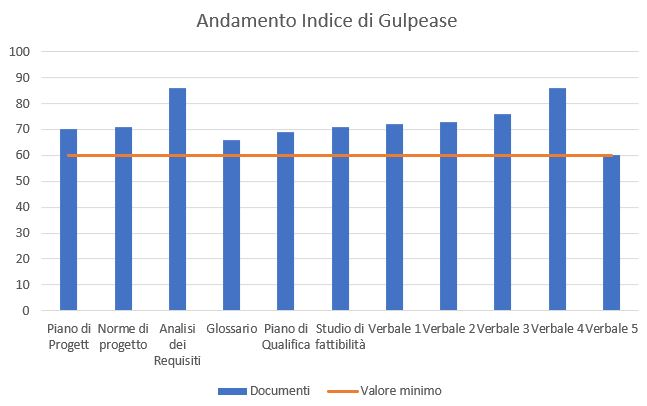
\includegraphics[width=12cm]{img/media_gul.jpg}
	\caption{ Andamento Indice di Gulpease}
\end{figure}

\paragraph{Considerazioni sui risultati e sull’esito della revisione }
I risultati ottenuti dall’esito della revisione sono stati poco soddisfacenti a livello personale, 
mentre i colloqui e commenti si sono rivelati essenziali e esaustici al fine di comprendere le modifiche da apportare
e soprattutto realizzare un prodotto migliore. \\
Dopo l'esito ci siamo resi conto degli errori e delle imperfezioni fatte, 
e come poter ovviare a questi in modo da produrre un prodotto migliore, vedi \S\ref{par:retrospettiva-RR}. \\


\subsection{Secondo periodo (RP)}
\label{sub:periodo-RP}
In questa sezione devo mettere gli esiti dei test fatti
\paragraph{Risultati test fase di progettazione architetturale}

\end{document}